\documentclass{senior-design}
\usepackage{lipsum}

%%% Report information %%%%%%%%%%%%%%%%%%%%%%%%%%%%%%%%%%%%%%%%%%
\reporttitle{An Awesome Project Made By An Amazing Team}
\reporttype{Individual Progress Report} % Uncomment this line if you want to use \generalreportcover
\semester{Spring 2023}
\sponsor{\name{Your}{Professor}}
\ta{\name{Hello}{World}}
\reportdate{\today}
\authornames{
    \nameemail{San}{Zhang}{sanz0@illinois.edu}\\[1em]
    \nameemail{Si}{Li}{sil0@illinois.edu}\\[1em]
    \nameemail{Dawu}{Wang}{dawu@example.com}\\[1em]
    \nameemail{English}{Member}{englishm0@illinois.edu}
}
\addbibresource{references.bib} % The bib database
%%%%%%%%%%%%%%%%%%%%%%%%%%%%%%%%%%%%%%%%%%%%%%%%%%%%%%%%%%%%%%%%%

%%% Uncomment the lines you need according to the type of report:
\projectnumber{114}
\teamnumber{514}
%%%%%%%%%%%%%%%%%%%%%%%%%%%%%%%%%%%%%%%%%%%%%%%%%%%%%%%%%%%%%%%%%

\begin{document}
%%% TITLE PAGE: select the one you need %%%%%%%%%%%%%%%%%%%%%%%%%
% \individualreportcover  % coverpage for individual report used for ZJU degree appl.
\generalreportcover % coverpage for other reports; NEEDS \reporttype{<Type>}
%%%%%%%%%%%%%%%%%%%%%%%%%%%%%%%%%%%%%%%%%%%%%%%%%%%%%%%%%%%%%%%%%
\frontmatter
%%% Abstract %%%%%%%%%%%%%%%%%%%%%%%%%%%%%%%%%%%%%%%%%%%%%%%%%%%%
\chapter*{Abstract}
Put your abstract here

\paragraph{Keywords}
% Put keywords below
Keyword 1, keyword 2, keyword 3

%%% TOC %%%%%%%%%%%%%%%%%%%%%%%%%%%%%%%%%%%%%%%%%%%%%%%%%%%%%%%%%
\tableofcontents
%%%%%%%%%%%%%%%%%%%%%%%%%%%%%%%%%%%%%%%%%%%%%%%%%%%%%%%%%%%%%%%%%

\mainmatter
%%% Body %%%%%%%%%%%%%%%%%%%%%%%%%%%%%%%%%%%%%%%%%%%%%%%%%%%%%%%%
\chapter{Introduction}
\section{Problem statement}
\lipsum[1]\cite{li1999,haynes1951}.
\section{Importance}
\begin{equation}
    f\left( x \right) =\sum_{n=0}^{\infty}{\frac{1}{n!}f^{\left( n \right)}\left( x_0 \right) \left( x-x_0 \right) ^n}, x\in U\left( x_0 \right)
\end{equation}
\begin{equation}
    \begin{aligned}
    e^{ix}&=1+ix+\frac{1}{2!}\left( ix \right) ^2+\frac{1}{3!}\left( ix \right) ^3+\cdots \frac{1}{n!}\left( ix \right) ^n+\cdots
    \\
    &=1+ix-\frac{1}{2!}x^2-i\frac{1}{3!}x^3+\frac{1}{4!}x^4+i\frac{1}{5!}x^5-\cdots
    \\
    &=\left( 1-\frac{1}{2!}x^2+\frac{1}{4!}x^4-\cdots \right) +i\left( x-\frac{1}{3!}x^3+\frac{1}{5!}x^5-\cdots \right)
    \\
    &=\cos x+i\sin x
    \end{aligned}
\end{equation}
\section{Literature Review}
\lipsum[2]\cite{j.a.prufrock2009,li1999,ref1}.

\begin{lstlisting}[language=c]
#include<stdio.h>
void fuzzy(int x){
    return x;
}
int main(){
    int a = 0, b, c;
    scanf("%d", &b);
    c = b;
    if (a == b)
        a = fuzzy(c);
    else
        b = fuzzy(a);
    printf("%d %d\n", a, fuzzy(c));
    return 0;
}
\end{lstlisting}

\chapter{Methodology}

Test the ability to print some units, say (in texts), \SI{10e5}{\um\ohm\degree}.

It also applies to equations,
\begin{equation}
    R_{t}=\SI{10e5}{\um\ohm\degree}
\end{equation}

\chapter{Results}
\begin{figure}[H]
    \centering
    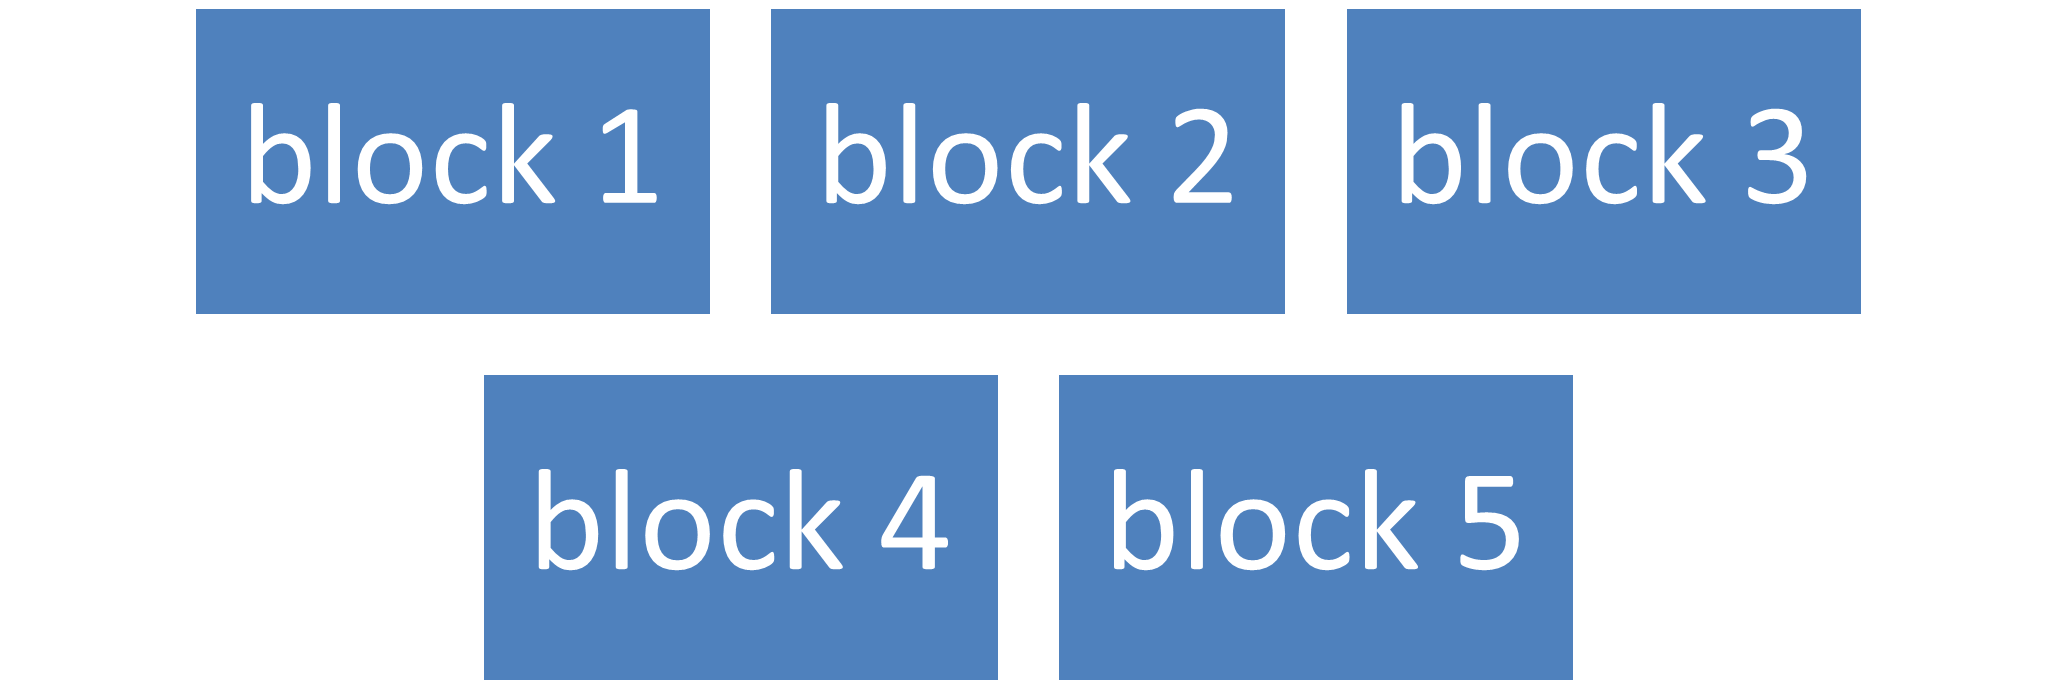
\includegraphics[width=0.8\linewidth]{figs/Picture1.png}
    \caption{An example figure.}
\end{figure}
\chapter{Discussion}

\chapter{Conclusion}

%%%%%%%%%%%%%%%%%%%%%%%%%%%%%%%%%%%%%%%%%%%%%%%%%%%%%%%%%%%%%%%%%

%%% References %%%%%%%%%%%%%%%%%%%%%%%%%%%%%%%%%%%%%%%%%%%%%%%%%%
\clearpage
\renewcommand*{\UrlFont}{\rmfamily}
\printbibliography[title={References},heading=bibintoc]
\clearpage
%%%%%%%%%%%%%%%%%%%%%%%%%%%%%%%%%%%%%%%%%%%%%%%%%%%%%%%%%%%%%%%%%
%%% Appendices %%%%%%%%%%%%%%%%%%%%%%%%%%%%%%%%%%%%%%%%%%%%%%%%%%
\begin{appendices}
% All appendices here, using sections for multiple appendices
\chapter{Example}
An example piece of code:
\lstinputlisting[language=python]{code/example.py}

\section{Some Test Data}

\section{Derivation of Square Law}
\end{appendices}
\clearpage
%%%%%%%%%%%%%%%%%%%%%%%%%%%%%%%%%%%%%%%%%%%%%%%%%%%%%%%%%%%%%%%%%
\backmatter
%%% Acknowledgement %%%%%%%%%%%%%%%%%%%%%%%%%%%%%%%%%%%%%%%%%%%%%
\chapter*{Acknowledgement}
Thank you thank you!
%%%%%%%%%%%%%%%%%%%%%%%%%%%%%%%%%%%%%%%%%%%%%%%%%%%%%%%%%%%%%%%%%
\end{document}